\documentclass[aspectratio=169]{beamer}

\usepackage{fontspec}
\usepackage{polyglossia}
\usepackage{color}
\usepackage{listings}
\setdefaultlanguage{russian}
\usepackage{csquotes}
\usetheme{metropolis}
\metroset{background=light}
\metroset{sectionpage=none}
\metroset{numbering=fraction}

\definecolor{ssaublue}{RGB}{77,144,205}
\setbeamercolor{frametitle}{fg=white, bg=ssaublue}
\setbeamercolor{title separator}{fg=ssaublue}

\setmainfont[
    Path = ../fonts/elektratextpro/,
    Extension = .otf,
    UprightFont = elektratextpro,
    BoldFont = elektratextpro_bold,
    ItalicFont = elektratextpro_italic,
    BoldItalicFont = elektratextpro_bolditalic
]{elektratextpro}

\setsansfont[
    Path = ../fonts/elektratextpro/,
    Extension = .otf,
    UprightFont = elektratextpro,
    BoldFont = elektratextpro_bold,
    ItalicFont = elektratextpro_italic,
    BoldItalicFont = elektratextpro_bolditalic
]{elektratextpro}

\setmonofont[
    Path = ../fonts/elektratextpro/,
    Extension = .otf,
    UprightFont = elektratextpro,
    BoldFont = elektratextpro_bold,
    ItalicFont = elektratextpro_italic,
    BoldItalicFont = elektratextpro_bolditalic
]{elektratextpro}

\newfontfamily\cyrillicfont[
    Path = ../fonts/elektratextpro/,
    Extension = .otf,
    UprightFont = elektratextpro,
    BoldFont = elektratextpro_bold,
    ItalicFont = elektratextpro_italic,
    BoldItalicFont = elektratextpro_bolditalic
]{elektratextpro}

\newfontfamily\cyrillicfontsf[
    Path = ../fonts/elektratextpro/,
    Extension = .otf,
    UprightFont = elektratextpro,
    BoldFont = elektratextpro_bold,
    ItalicFont = elektratextpro_italic,
    BoldItalicFont = elektratextpro_bolditalic
]{elektratextpro}

\newfontfamily\cyrillicfonttt[
    Path = ../fonts/elektratextpro/,
    Extension = .otf,
    UprightFont = elektratextpro,
    BoldFont = elektratextpro_bold,
    ItalicFont = elektratextpro_italic,
    BoldItalicFont = elektratextpro_bolditalic
]{elektratextpro}

% Настройка листингов для Beamer
\lstset{
    basicstyle=\ttfamily\footnotesize,
    commentstyle=\color{gray},
    columns=fullflexible,
    keepspaces=true,
    breaklines=false,
    extendedchars=true,
    texcl=true,
    showstringspaces=false
}
\usepackage{svg}

\title{Docker Compose}
\date{29 октября 2025 г.}

\begin{document}

\maketitle

\begin{frame}{Развитие приложения: новое требование}
\textbf{Текущее состояние нашего приложения:}

\begin{itemize}
\item nginx работает в контейнере и раздает html
\item Сервер настраивается через ansible
\item Настроен автоматический деплой через CI/CD pipeline
\end{itemize}

\vspace{0.3cm}

\textbf{Новое требование:}

Добавить API для работы с динамическими данными. Важный критерий — высокая доступность.
\end{frame}

\begin{frame}{Целевая архитектура}
%@startuml
%actor "Пользователь" as User
%
%rectangle "Nginx" as Nginx
%rectangle "Backend 1" as Backend1
%rectangle "Backend 2" as Backend2
%rectangle "Backend 3" as Backend3
%
%User -right-> Nginx : HTTP запросы
%Nginx -left-> User : Статические файлы\n(HTML, CSS, JS)
%Nginx -down-> Backend1 : /api/* запросы
%Nginx -down-> Backend2
%Nginx -down-> Backend3
%@enduml
\begin{figure}
\centering
\includesvg{lb-schema}
\label{fig:lb-schema}
\end{figure}
\end{frame}

\section{Вызовы многоконтейнерной архитектуры}

\begin{frame}{Что нам нужно запустить?}
\textbf{Для реализации нашей архитектуры потребуется:}

\begin{itemize}
\item \textbf{1 nginx контейнер} — веб-сервер и load balancer
\item \textbf{3 backend контейнера} — Python Flask API
\item \textbf{Docker сеть} — для связи между контейнерами
\end{itemize}

\vspace{0.3cm}

Как это запустить?
\end{frame}

\begin{frame}[fragile]{Попробуем запустить вручную}
\textbf{Последовательность команд:}

\begin{verbatim}
docker network create demo-net
docker run -d --rm --network demo-net --name backend-1 busybox:stable sleep 250
docker run -d --rm --network demo-net --name backend-2 busybox:stable sleep 250
docker run -d --rm --network demo-net --name backend-3 busybox:stable sleep 250
docker run -d --rm --network demo-net -p 8080:80 --name nginx nginx:alpine
\end{verbatim}

\vspace{0.2cm}

\textbf{Проблемы:} много команд, можно ошибиться
\end{frame}

\section{Docker Compose как решение}

\begin{frame}{Docker Compose}
\textbf{Docker Compose} — инструмент для определения и запуска многоконтейнерных приложений

\vspace{0.2cm}

\textbf{Ключевые возможности:}
\begin{itemize}
\item \textbf{Декларативное описание} — вся архитектура в одном YAML файле
\item \textbf{Простое управление} — одна команда для запуска всего стека
\item \textbf{Автоматическое масштабирование} — легко увеличить количество экземпляров
\item \textbf{Управление зависимостями} — контейнеры запускаются в правильном порядке
\end{itemize}

\vspace{0.2cm}

\textbf{Результат:} вместо N команд docker — одна команда
\end{frame}

\section{Основные команды}

\begin{frame}{Команды жизненного цикла}
  \textbf{Основные команды Docker Compose:}

  \begin{itemize}
    \item \textbf{docker compose up} — запустить все сервисы
    \item \textbf{docker compose up -d} — запустить в фоновом режиме
    \item \textbf{docker compose down} — остановить и удалить контейнеры
    \item \textbf{docker compose build} — пересобрать образы
    \item \textbf{docker compose pull} — загрузить новые версии образов
  \end{itemize}

  \vspace{0.2cm}

  \textbf{Команды мониторинга:}
  \begin{itemize}
    \item \textbf{docker compose ps} — статус всех сервисов
    \item \textbf{docker compose logs} — логи всех сервисов
  \end{itemize}
\end{frame}


\begin{frame}[fragile]{Масштабирование в Compose}
\href{https://docs.docker.com/compose/how-tos/environment-variables/envvars/#project-and-file-configuration}{Имя контейнера}: \texttt{<project-name>-<service>-\#}
\vspace{0.2cm}

\begin{verbatim}
docker compose up -p app --scale backend=3
\end{verbatim}

\vspace{0.2cm}

Будут созданы три контейнера:
\begin{verbatim}
app-backend-1
app-backend-2
app-backend-3
\end{verbatim}
\end{frame}

\begin{frame}{Много других возможностей}

\begin{itemize}
  \item \href{https://docs.docker.com/compose/compose-file/06-networks/}{Сети} — изоляция и связь между сервисами
  \item \href{https://docs.docker.com/compose/use-secrets/}{Секреты} — безопасное управление паролями и ключами
  \item \href{https://docs.docker.com/compose/compose-file/07-volumes/}{Volumes} — постоянное хранение данных
  \item \href{https://docs.docker.com/compose/compose-file/05-services/\#healthcheck}{Health checks} — мониторинг состояния сервисов
  \item \href{https://docs.docker.com/compose/compose-file/05-services/\#depends_on}{Зависимости} — контроль порядка запуска сервисов
\end{itemize}
\vspace{0.3cm}

\textbf{Полная документация:} \href{https://docs.docker.com/compose/}{docs.docker.com/compose/}
\end{frame}

\begin{frame}{Несколько Docker Compose файлов}
  \begin{center}
    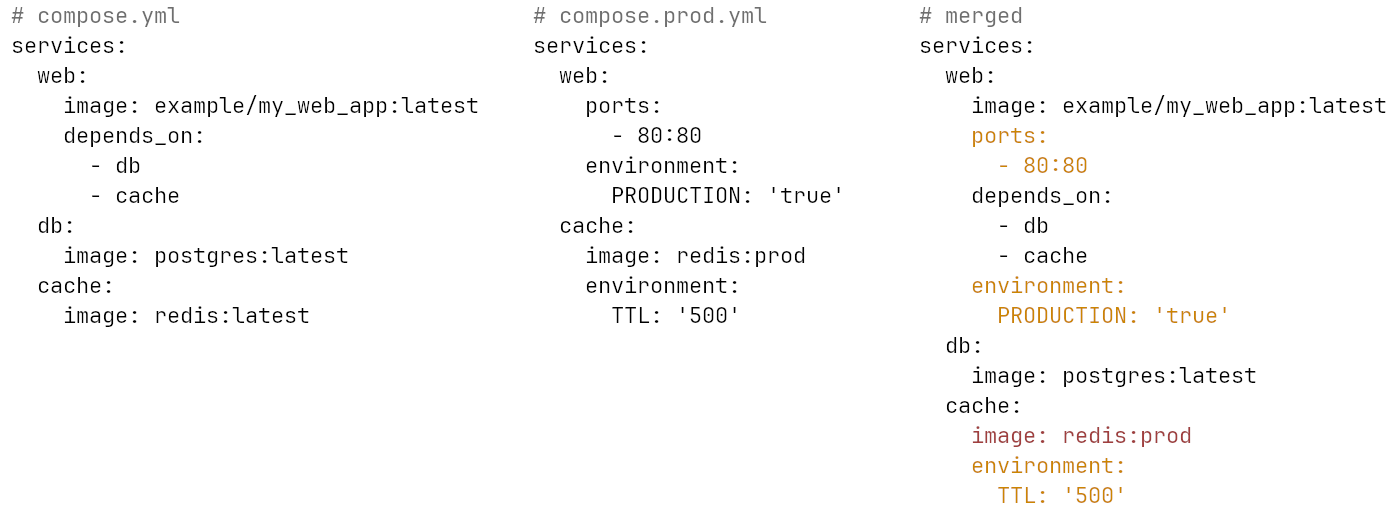
\includegraphics[width=1\textwidth]{media/compose-merge}
  \end{center}

  \footnotesize{\textcolor{gray}{\url{https://docs.docker.com/compose/how-tos/multiple-compose-files/}}}
\end{frame}

\begin{frame}{Демонстрация: Docker Compose}
  \textbf{Что покажем:}
  \begin{enumerate}
    \item Настройка docker compose файла для схемы из начала лекции
    \item Работа с несколькими файлами docker compose
  \end{enumerate}

  \vspace{0.2cm}

  \textbf{Демо-репозиторий:} \\
  \href{https://github.com/prafdin/devops-demo-website/tree/compose-demo}{\texttt{https://github.com/prafdin/devops-demo-website/tree/compose-demo}}

\end{frame}

\begin{frame}{Альтернативы Docker Compose}

\begin{itemize}
  \item \textbf{Docker Swarm} — расширение функционала docker compose
  \item \textbf{Nomad} — от HashiCorp, поддерживает не только контейнеры
  \item \textbf{Kubernetes} — индустриальный стандарт оркестрации
  \item \textbf{OpenShift} — enterprise платформа на базе Kubernetes
\end{itemize}

\end{frame}

\begin{frame}{Docker Swarm}
  \begin{center}
    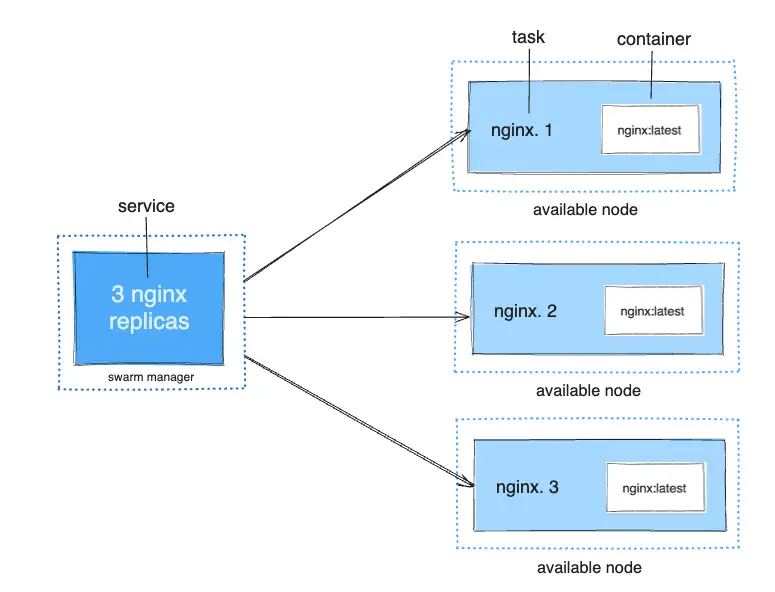
\includegraphics[width=0.65\textwidth]{media/swarm}
  \end{center}
\end{frame}

\begin{frame}{Kubernetes}
  \begin{center}
    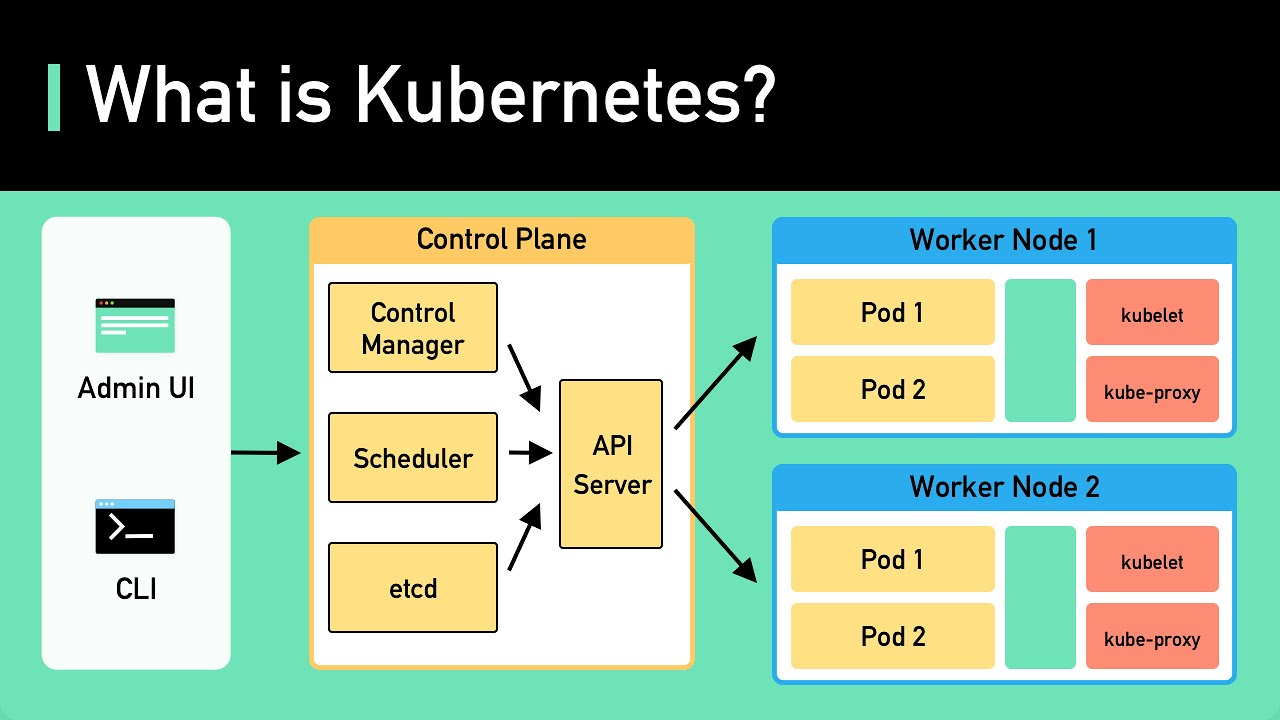
\includegraphics[width=0.8\textwidth]{media/kuber}
  \end{center}
\end{frame}

\section{Заключение}

\begin{frame}{Что запомнить}
  \begin{itemize}
    \item Docker Compose решает проблему сложности управления множеством связанных контейнеров
    \item Декларативный подход лучше императивного — надёжнее и проще в поддержке
  \end{itemize}

  \vspace{1cm}
  \begin{center}
    \textbf{Вопросы?}
  \end{center}
\end{frame}
\end{document}